\chapter{Optimization methodology}
Given a cost/objective function $f: \mathcal{X} \rightarrow \mathbb{R}$, where the domain
$\mathcal{X}$ could be a subset of $\mathbb{R}^n$,
optimization is a methodology which seeks to find an optimal point, $x^*$, and value
$f^* = f(x)$, given as
\begin{align}\label{OPT}
    x^* \in \arg\min_{x \in \mathcal{X}} f(x) \hspace{1cm} f^* = \min_{x \in \mathcal{X}} f(x) = f(x^*).
\end{align}
Note that the above formulation is a minimization problem, which is equivalent to a
maximization problem maximizing $-f(\cdot)$. Throughout this thesis, we choose to only work
with a minimization problem. 
Solving this problem is intractable except for rare cases e.g. if $f$ is 
convex and analytically directly solvable or the domain of $f$ is very limited. Hm

\begin{testexample}[Direct solution method]
    The unconstrained linear least squares, $$\min_{x\in \mathbb{R}^n} f(x) := ||Ax-b||_2^2$$
    where $A \in \mathbb{R}^{m\times n}$ and $b \in \mathbb{R}^m$, is a convex problem,
    i.e. finding $x^*$ such that $\nabla f(x^*) = 0$ is equivalent to finding the solution
    to the problem. Assuming $A^TA$ is invertable, linear least squares can be solved
    directly by the normal equations, 
    $$\nabla f(x) = 2A^TAx + 2b^TA = 0 \hspace{0.5cm} \Leftrightarrow \hspace{0.5cm} x^* = (A^TA)^{-1} A^Tb$$
\end{testexample}

Most optimization problems are non-convex with multiple local minima. And even if the gradient is
given analytically the solution is found among a potentially infinitely large 
set of stationary points ($\nabla f(x) = 0$) and boundary points - this might be tedious or impossible.
When the problem is not directly solvable, mathematical optimization takes an indirect methodology: 
Design a sequence of experiments that reveal information of the objective function. This information 
can hopefully lead us to the solution of \eqref{OPT}. This general way of sequentially solving 
is presented in the book Bayesian Optimization by Roman Garnett \cite{bayesoptbook} and 
presented here as Algorithm \ref{algOPT}. 
W
\begin{algorithm}
\caption{Sequencial Optimization \cite{bayesoptbook} }\label{algOPT}
\begin{algorithmic}
\State \textbf{Input:} Initial dataset $\mathcal{D}$  \Comment{can be empty}
\While{Temination is not reached}
    \State $x \gets \text{policy}(\mathcal{D})$ \Comment{select next observation location}
    \State $y \gets \text{observe}(x)$ \Comment{observe objective function at chosen location}
    \State $\mathcal{D} \gets \mathcal{D} \cup \{(x,y)\} $ \Comment{update dataset}
\EndWhile
\State $\textbf{return: } \mathcal{D}$
\end{algorithmic}
\end{algorithm}

Given data points in the optimization landscape\footnote{"Optimization landscape" defined as the joint set of points in the domain and the objective function
evaluated in the points, i.e. $\{(x,f(x))\in \mathcal{X} \times \mathbb{R}| x \in \mathcal{X}\}$} 
a policy selects a point $x \in \mathcal{X}$ where we make our next observation. Policies can be deterministic or probibalitic, e.g. 
grid search and random search are examples of policies. The next observation provides us a $y$ value, which combined with $x$ is included to the 
available data $\mathcal{D}$. Finaly, a stopping criterion decides whether to continue or terminate. 

<example of random search is half as efficient as BO>


\begin{testexample}[Grid search]
    In grid search values along each dimention in $\mathcal{X}$ is seleced and combined with each
    other, which thereby defines a grid in the parameter space. All points are ordered and systematicly
    selected. In the content of algorhtim \ref{algOPT} we define the grid search policy as 
    $$\text{policy}_{GS}(\mathcal{D}) = x_{|\mathcal{D}|+1}$$
    assuming $x_1,x_2, \dots, x_{n}$ are the ordered grid points and the size of the obtained 
    data is $|\mathcal{D}|$. 
\end{testexample}
\begin{testexample}[Random search]
    In random search a uniform distribtuion is layed over the domain space $\mathcal{X}$ and a random point
    is selected from the distribtuion. 
    $$\text{policy}_{RS}(\mathcal{D}) = x, \hspace{0.5cm} x \sim p(\mathcal{X})$$
    Note that grid search and random search are policies which completely 
    ignores the available data. This is a shame and we can do better. 
\end{testexample}

\begin{testexample}[Gradient descent]
    Gradient descent is the most simple gradient-based optimization approach. The gradient of a continuous 
    function points in the most ascending direction from the location where it is evaluated.
    In the minimization task, \eqref{OPT}, we can iteratively use the opposite gradient direction, i.e. the most 
    descenting directiong. This yields the policy:
    $$\text{policy}_{GD}(\mathcal{D}) = x_n - \eta \nabla f(x_n)$$
    where we for a brief moment modify $y$ to be a vector, since the observation model 
    is given as:
    $$\text{observe}_{GD}(x) = [f(x), \nabla f(x)]$$
\end{testexample}

\begin{testexample}[Surrogate-based optimization]
    <SVR> <Radial Basis function> <Polynomal model/respons surface>
    In surrogate-based optimization all available data is fitted by a cheap-to-evaluate approximation
    to the objective function - this approximation is called a \textit{surrogate} model. Examples
    of surrogate models could be a neural network or a random forest. The next point is 
    chosen as the point where the surrogate model is minimized. 
    $$\text{policy}_{sur}(\mathcal{D}) = \min_x \hat f(x)$$
    where $\hat f(x) \approx f(x)$ for $x$ close to the data $\mathcal{D}$. And we hope the approximation
    holds for $x$ far away from the the data. 
\end{testexample}

\section{When to use Bayesian optmization}
What if $f(x)$ took serval days to evaluate. What if $f(x)$ is noisy? what if discrete points? 
<more here>

% \begin{figure}[h]
%     \centering
%     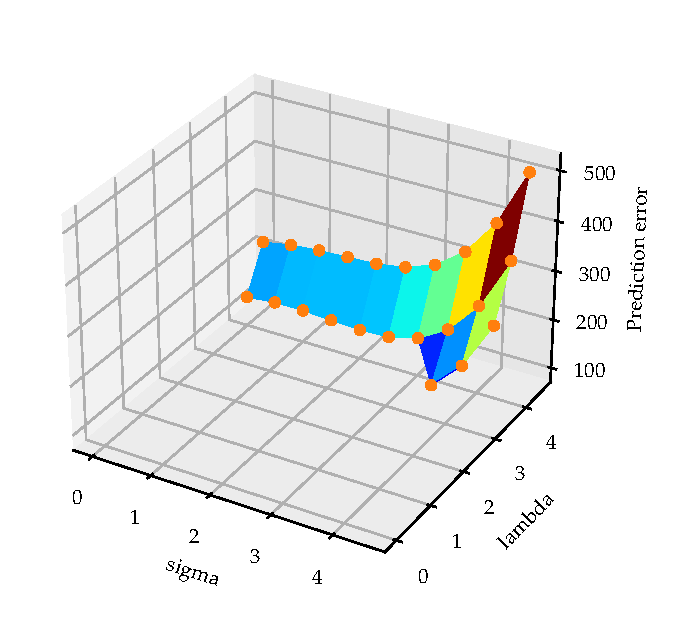
\includegraphics[width=0.9\textwidth]{Pictures/BO_vs_Grid2.eps}
%     \caption{Hyper parameter tuning of a model $M(\lambda, \sigma)$, 
%     35 evaluation in grid search vs 39 evaluations using Bayesian optimization}
%     \label{optimhist}
% \end{figure}

\begin{figure}[H]%
    \centering
    {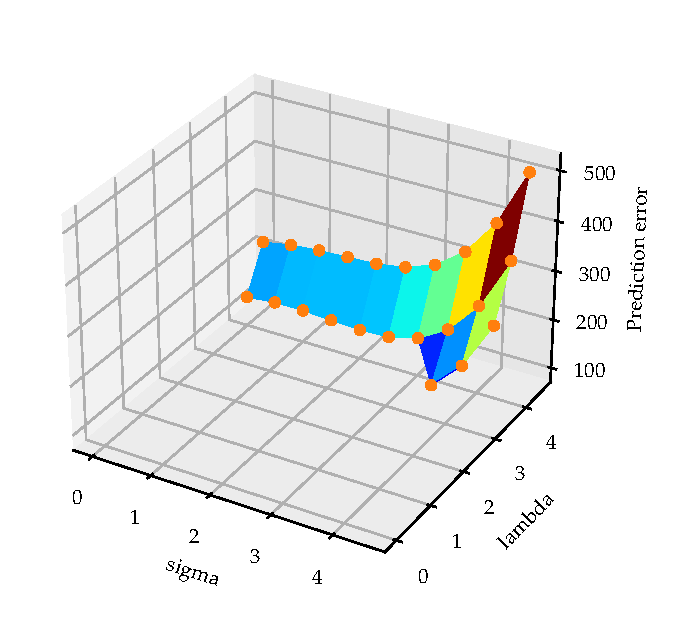
\includegraphics[width=0.46\textwidth]{Pictures/BO_vs_Grid2.eps} }%
    \qquad
   {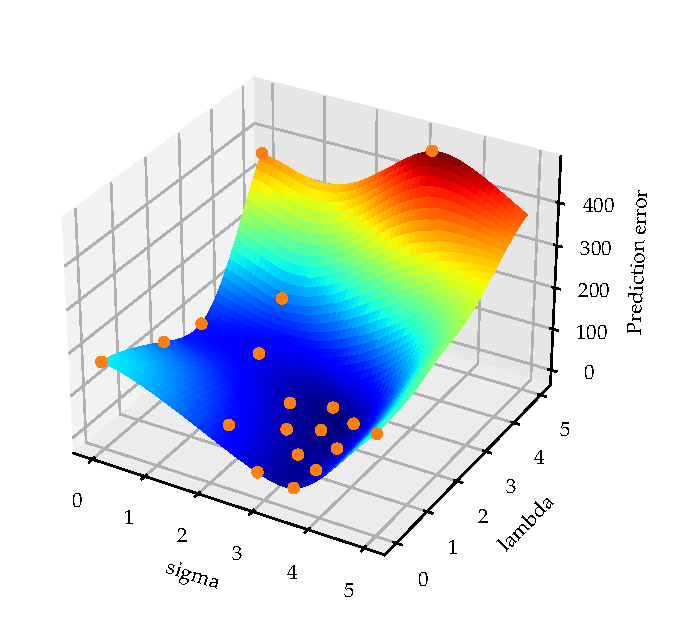
\includegraphics[width=0.46\textwidth]{Pictures/BO_vs_Grid1.eps} }%
    \caption{Hyper parameter tuning of a model $M(\lambda, \sigma)$, 
    23 evaluation in grid search vs 23 evaluations using Bayesian optimization}%
    \label{fig:example}%
\end{figure}


additionally, Bayesian Optimization allow for observation noise, 

\section{Observation model}\label{ObsModel}
Many optimization algorithms assume \textit{exact} evaluations of the objective function. However, this assumption
is often wrong especially for objective functions with real-life experiments, imperfect simulations, human interaction 
where measurement noise is a well known. The observation model is typically noisy and described as
$$y = f(x)+\epsilon$$ where $\epsilon$ is the measurement error, this is
typically assumed to be Gaussian with zero mean and a variance
$\sigma^2$ (which could depend on $x$ in a heterostodatic setting) and implies a Gaussian observation model, 
$$p(y|x,f(x),\sigma) = \mathcal{N}(y;f(x),\sigma^2)$$ 

% (note from now on we define $\phi := f(x)$ in order to avoid confusion and a extra set of paranteses)
% $$p(y|x,\phi,\sigma) = \mathcal{N}(y;\phi,\sigma^2)$$ 
we can extend this model to deal with noiseless observations as well, simply by setting $\sigma = 0$ and let the
model colaps into a Direct delta distribution, 
$$p(y|x, f(x)) = \mathcal{\delta}(y-f(x))$$
i.e. all probability mass for $y$ is on the value $f(x)$ giving the observation sample $y = f(x)$


